\documentclass{standalone}
\usepackage{tikz}
\usetikzlibrary{patterns, positioning}
\usepackage[sfdefault]{ClearSans} %% option 'sfdefault' activates Clear Sans as the default text font
\usepackage[T1]{fontenc}

\begin{document}
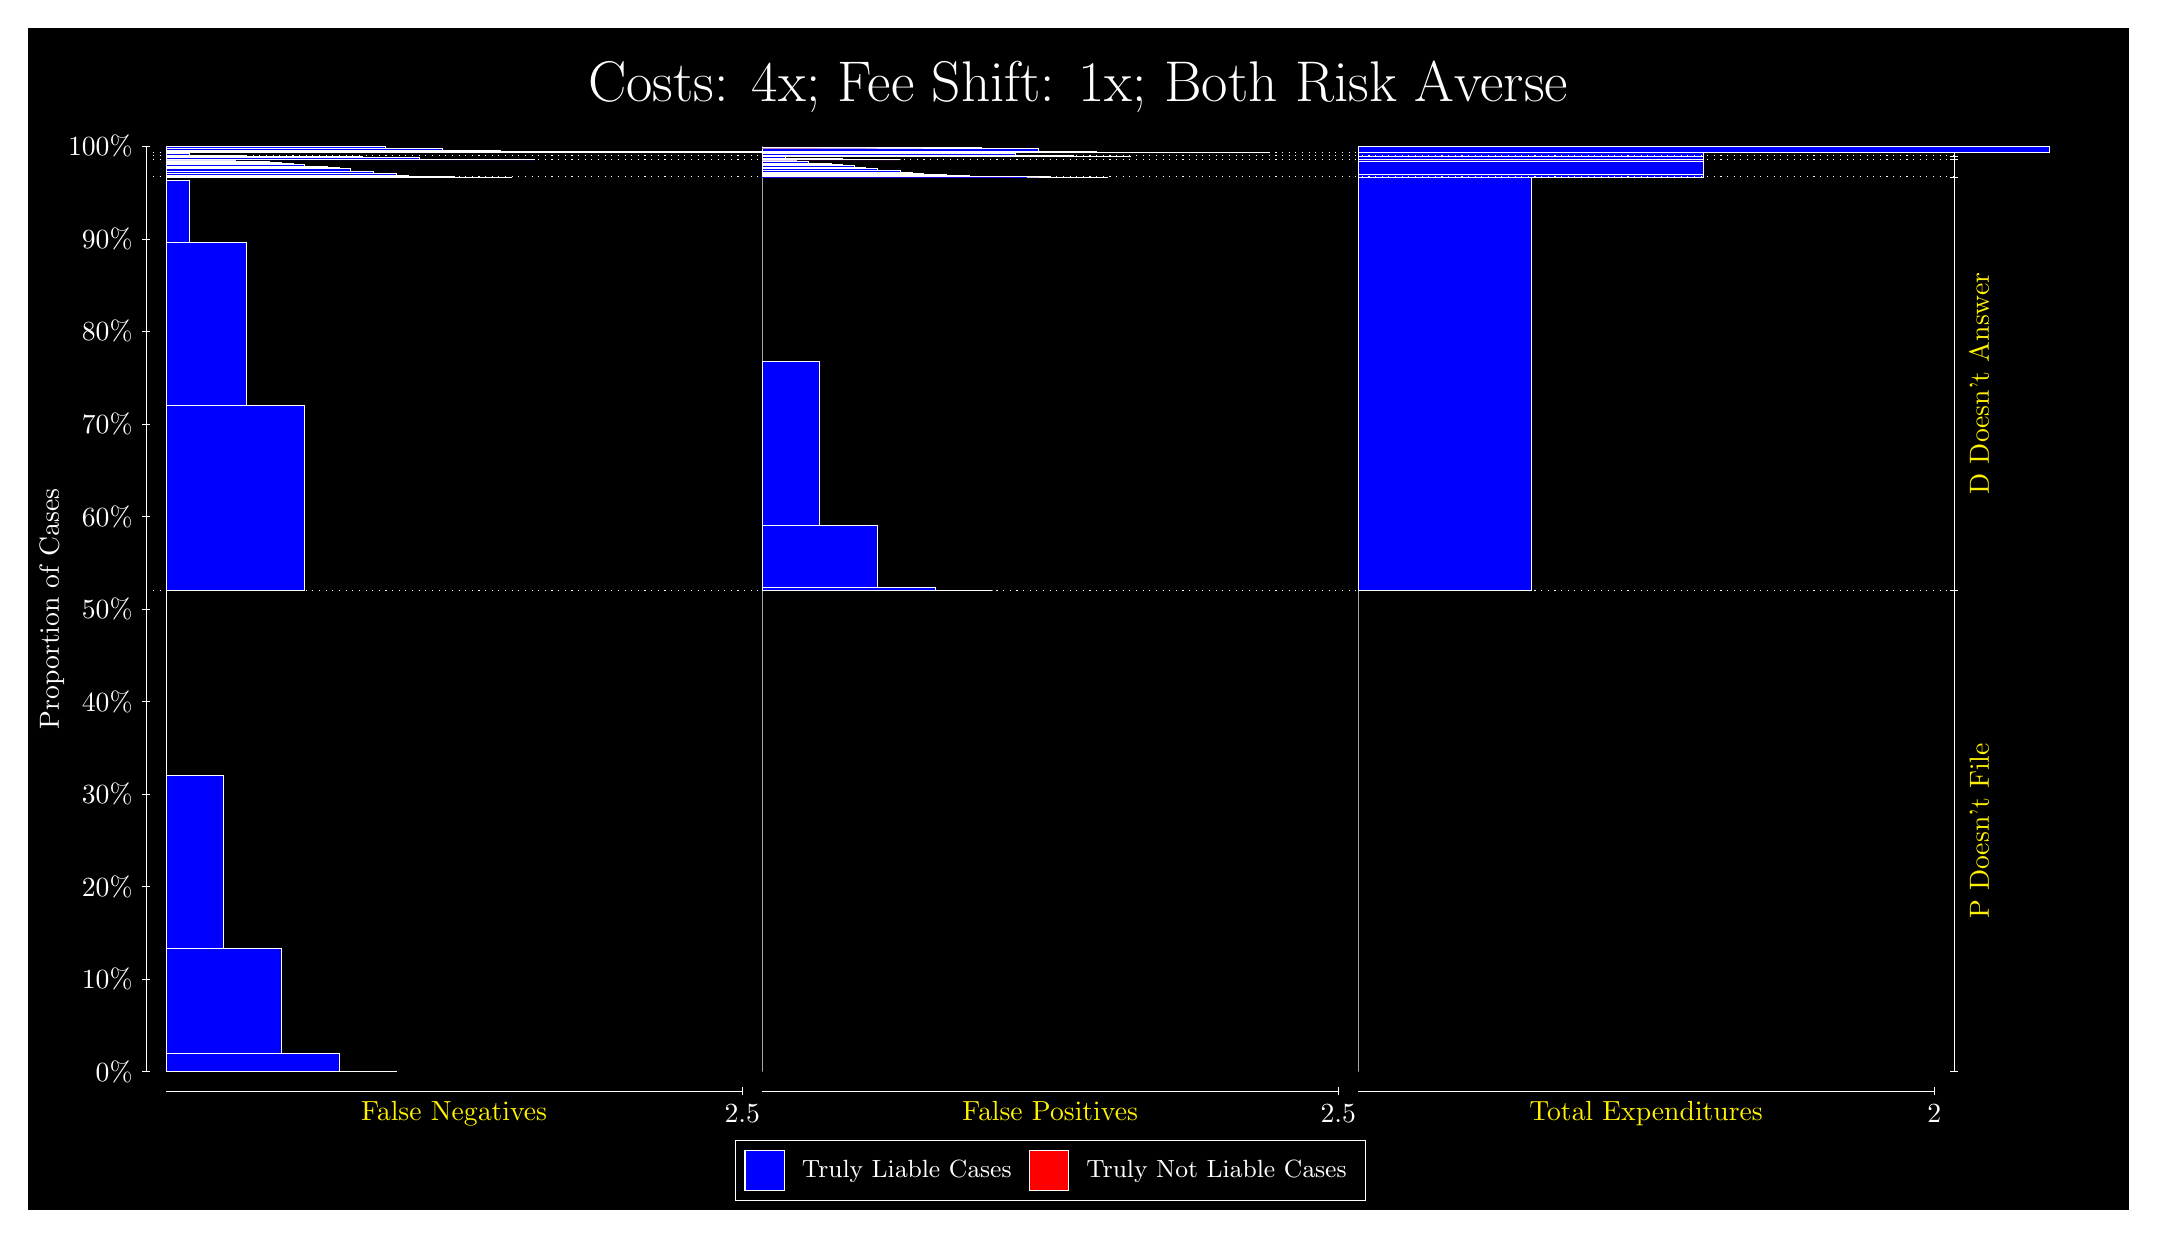
\begin{tikzpicture}
\draw[fill=black] (0,0) rectangle (26.667,15);
\draw[text=white] (0,13.5) rectangle (26.667,15) node[midway] {\huge Costs: 4x; Fee Shift: 1x; Both Risk Averse};
\draw[white, very thin] (1.5,1.75) -- (1.5,13.5);
\node[rotate=90, text=white, anchor=center] at (0.3, 7.625) {Proportion of Cases};
\draw[white, very thin] (1.45,1.75) -- (1.55,1.75);
\node[text=white, anchor=east] at (1.45, 1.75) {0\%};
\draw[white, very thin] (1.45,2.925) -- (1.55,2.925);
\node[text=white, anchor=east] at (1.45, 2.925) {10\%};
\draw[white, very thin] (1.45,4.1) -- (1.55,4.1);
\node[text=white, anchor=east] at (1.45, 4.1) {20\%};
\draw[white, very thin] (1.45,5.275) -- (1.55,5.275);
\node[text=white, anchor=east] at (1.45, 5.275) {30\%};
\draw[white, very thin] (1.45,6.45) -- (1.55,6.45);
\node[text=white, anchor=east] at (1.45, 6.45) {40\%};
\draw[white, very thin] (1.45,7.625) -- (1.55,7.625);
\node[text=white, anchor=east] at (1.45, 7.625) {50\%};
\draw[white, very thin] (1.45,8.8) -- (1.55,8.8);
\node[text=white, anchor=east] at (1.45, 8.8) {60\%};
\draw[white, very thin] (1.45,9.975) -- (1.55,9.975);
\node[text=white, anchor=east] at (1.45, 9.975) {70\%};
\draw[white, very thin] (1.45,11.15) -- (1.55,11.15);
\node[text=white, anchor=east] at (1.45, 11.15) {80\%};
\draw[white, very thin] (1.45,12.325) -- (1.55,12.325);
\node[text=white, anchor=east] at (1.45, 12.325) {90\%};
\draw[white, very thin] (1.45,13.5) -- (1.55,13.5);
\node[text=white, anchor=east] at (1.45, 13.5) {100\%};

\draw[white, very thin] (24.457,1.75) -- (24.457,13.5);
\draw[white, very thin] (24.407,1.75) -- (24.507,1.75);
\node[anchor=west] at (24.407, 1.75) {};
\draw[white, very thin] (24.407,7.8603) -- (24.507,7.8603);
\node[anchor=west] at (24.407, 7.8603) {};
\draw[white, very thin] (24.407,13.113) -- (24.507,13.113);
\node[anchor=west] at (24.407, 13.113) {};
\draw[white, very thin] (24.407,13.331) -- (24.507,13.331);
\node[anchor=west] at (24.407, 13.331) {};
\draw[white, very thin] (24.407,13.378) -- (24.507,13.378);
\node[anchor=west] at (24.407, 13.378) {};
\draw[white, very thin] (24.407,13.423) -- (24.507,13.423);
\node[anchor=west] at (24.407, 13.423) {};
\draw[white, very thin] (24.407,13.5) -- (24.507,13.5);
\node[anchor=west] at (24.407, 13.5) {};

\draw[white, very thin, fill=blue] (1.75,1.75) rectangle (4.6775,1.7523);
\draw[white, very thin, fill=blue] (1.75,1.7523) rectangle (3.9457,1.9776);
\draw[white, very thin, fill=blue] (1.75,1.9776) rectangle (3.2138,3.313);
\draw[white, very thin, fill=blue] (1.75,3.313) rectangle (2.4819,5.5118);
\draw[white, very thin, fill=red] (1.75,5.5118) rectangle (1.75,5.5118);
\draw[white, very thin, fill=blue] (1.75,5.5118) rectangle (1.75,7.8603);
\draw[white, very thin, fill=blue] (1.75,7.8603) rectangle (3.5065,10.207);
\draw[white, very thin, fill=blue] (1.75,10.207) rectangle (2.7746,12.286);
\draw[white, very thin, fill=blue] (1.75,12.286) rectangle (2.0428,13.075);
\draw[white, very thin, fill=red] (1.75,13.075) rectangle (1.75,13.075);
\draw[white, very thin, fill=blue] (1.75,13.075) rectangle (1.75,13.113);
\draw[white, very thin, fill=blue] (1.75,13.113) rectangle (6.1413,13.113);
\draw[white, very thin, fill=blue] (1.75,13.113) rectangle (5.8486,13.113);
\draw[white, very thin, fill=blue] (1.75,13.113) rectangle (5.5558,13.113);
\draw[white, very thin, fill=blue] (1.75,13.113) rectangle (5.4094,13.117);
\draw[white, very thin, fill=blue] (1.75,13.117) rectangle (5.2631,13.117);
\draw[white, very thin, fill=blue] (1.75,13.117) rectangle (5.1167,13.124);
\draw[white, very thin, fill=blue] (1.75,13.124) rectangle (4.9703,13.124);
\draw[white, very thin, fill=blue] (1.75,13.124) rectangle (4.8239,13.131);
\draw[white, very thin, fill=blue] (1.75,13.131) rectangle (4.6775,13.155);
\draw[white, very thin, fill=blue] (1.75,13.155) rectangle (4.5312,13.16);
\draw[white, very thin, fill=blue] (1.75,13.16) rectangle (4.3848,13.16);
\draw[white, very thin, fill=blue] (1.75,13.16) rectangle (4.3848,13.178);
\draw[white, very thin, fill=blue] (1.75,13.178) rectangle (4.2384,13.185);
\draw[white, very thin, fill=blue] (1.75,13.185) rectangle (4.092,13.215);
\draw[white, very thin, fill=blue] (1.75,13.215) rectangle (4.092,13.215);
\draw[white, very thin, fill=blue] (1.75,13.215) rectangle (3.9457,13.228);
\draw[white, very thin, fill=blue] (1.75,13.228) rectangle (3.7993,13.245);
\draw[white, very thin, fill=blue] (1.75,13.245) rectangle (3.6529,13.247);
\draw[white, very thin, fill=blue] (1.75,13.247) rectangle (3.6529,13.252);
\draw[white, very thin, fill=blue] (1.75,13.252) rectangle (3.5065,13.273);
\draw[white, very thin, fill=blue] (1.75,13.273) rectangle (3.3602,13.286);
\draw[white, very thin, fill=blue] (1.75,13.286) rectangle (3.3602,13.287);
\draw[white, very thin, fill=blue] (1.75,13.287) rectangle (3.2138,13.299);
\draw[white, very thin, fill=blue] (1.75,13.299) rectangle (3.0674,13.3);
\draw[white, very thin, fill=blue] (1.75,13.3) rectangle (3.0674,13.304);
\draw[white, very thin, fill=blue] (1.75,13.304) rectangle (2.921,13.31);
\draw[white, very thin, fill=blue] (1.75,13.31) rectangle (2.921,13.31);
\draw[white, very thin, fill=blue] (1.75,13.31) rectangle (2.7746,13.316);
\draw[white, very thin, fill=blue] (1.75,13.316) rectangle (2.6283,13.316);
\draw[white, very thin, fill=blue] (1.75,13.316) rectangle (2.6283,13.319);
\draw[white, very thin, fill=blue] (1.75,13.319) rectangle (2.4819,13.323);
\draw[white, very thin, fill=blue] (1.75,13.323) rectangle (2.3355,13.323);
\draw[white, very thin, fill=blue] (1.75,13.323) rectangle (2.3355,13.326);
\draw[white, very thin, fill=blue] (1.75,13.326) rectangle (2.1891,13.328);
\draw[white, very thin, fill=blue] (1.75,13.328) rectangle (2.0428,13.328);
\draw[white, very thin, fill=blue] (1.75,13.328) rectangle (1.8964,13.329);
\draw[white, very thin, fill=red] (1.75,13.329) rectangle (1.75,13.329);
\draw[white, very thin, fill=blue] (1.75,13.329) rectangle (1.75,13.331);
\draw[white, very thin, fill=blue] (1.75,13.331) rectangle (6.4341,13.331);
\draw[white, very thin, fill=blue] (1.75,13.331) rectangle (5.7022,13.333);
\draw[white, very thin, fill=blue] (1.75,13.333) rectangle (4.9703,13.359);
\draw[white, very thin, fill=blue] (1.75,13.359) rectangle (4.2384,13.378);
\draw[white, very thin, fill=blue] (1.75,13.378) rectangle (3.5065,13.378);
\draw[white, very thin, fill=red] (1.75,13.378) rectangle (1.75,13.378);
\draw[white, very thin, fill=blue] (1.75,13.378) rectangle (3.5065,13.378);
\draw[white, very thin, fill=blue] (1.75,13.378) rectangle (2.7746,13.385);
\draw[white, very thin, fill=blue] (1.75,13.385) rectangle (2.0428,13.412);
\draw[white, very thin, fill=red] (1.75,13.412) rectangle (1.75,13.412);
\draw[white, very thin, fill=blue] (1.75,13.412) rectangle (1.75,13.423);
\draw[white, very thin, fill=blue] (1.75,13.423) rectangle (11.704,13.423);
\draw[white, very thin, fill=blue] (1.75,13.423) rectangle (10.972,13.423);
\draw[white, very thin, fill=blue] (1.75,13.423) rectangle (10.24,13.424);
\draw[white, very thin, fill=blue] (1.75,13.424) rectangle (9.508,13.434);
\draw[white, very thin, fill=blue] (1.75,13.434) rectangle (8.7761,13.437);
\draw[white, very thin, fill=blue] (1.75,13.437) rectangle (8.0442,13.438);
\draw[white, very thin, fill=blue] (1.75,13.438) rectangle (7.4587,13.438);
\draw[white, very thin, fill=blue] (1.75,13.438) rectangle (7.3123,13.438);
\draw[white, very thin, fill=blue] (1.75,13.438) rectangle (6.7268,13.438);
\draw[white, very thin, fill=blue] (1.75,13.438) rectangle (5.9949,13.446);
\draw[white, very thin, fill=blue] (1.75,13.446) rectangle (5.2631,13.481);
\draw[white, very thin, fill=blue] (1.75,13.481) rectangle (4.5312,13.498);
\draw[white, very thin, fill=blue] (1.75,13.498) rectangle (3.7993,13.5);
\draw[white, very thin, fill=blue] (1.75,13.5) rectangle (3.0674,13.5);
\draw[white, very thin, fill=blue] (1.75,13.5) rectangle (2.3355,13.5);
\draw[white, very thin, fill=red] (1.75,13.5) rectangle (1.75,13.5);
\draw[white, very thin, fill=red] (9.3189,1.75) rectangle (9.3189,1.75);
\draw[white, very thin, fill=blue] (9.3189,1.75) rectangle (9.3189,7.8603);
\draw[white, very thin, fill=red] (9.3189,7.8603) rectangle (12.246,7.8603);
\draw[white, very thin, fill=blue] (9.3189,7.8603) rectangle (12.246,7.8603);
\draw[white, very thin, fill=blue] (9.3189,7.8603) rectangle (11.515,7.8986);
\draw[white, very thin, fill=blue] (9.3189,7.8986) rectangle (10.783,8.688);
\draw[white, very thin, fill=blue] (9.3189,8.688) rectangle (10.051,10.766);
\draw[white, very thin, fill=blue] (9.3189,10.766) rectangle (9.3189,13.113);
\draw[white, very thin, fill=red] (9.3189,13.113) rectangle (13.71,13.113);
\draw[white, very thin, fill=blue] (9.3189,13.113) rectangle (13.71,13.113);
\draw[white, very thin, fill=red] (9.3189,13.113) rectangle (13.417,13.113);
\draw[white, very thin, fill=blue] (9.3189,13.113) rectangle (13.417,13.113);
\draw[white, very thin, fill=red] (9.3189,13.113) rectangle (13.125,13.113);
\draw[white, very thin, fill=blue] (9.3189,13.113) rectangle (13.125,13.113);
\draw[white, very thin, fill=blue] (9.3189,13.113) rectangle (12.978,13.115);
\draw[white, very thin, fill=red] (9.3189,13.115) rectangle (12.832,13.115);
\draw[white, very thin, fill=blue] (9.3189,13.115) rectangle (12.832,13.115);
\draw[white, very thin, fill=blue] (9.3189,13.115) rectangle (12.686,13.116);
\draw[white, very thin, fill=red] (9.3189,13.116) rectangle (12.539,13.116);
\draw[white, very thin, fill=blue] (9.3189,13.116) rectangle (12.539,13.116);
\draw[white, very thin, fill=blue] (9.3189,13.116) rectangle (12.393,13.118);
\draw[white, very thin, fill=red] (9.3189,13.118) rectangle (12.246,13.118);
\draw[white, very thin, fill=blue] (9.3189,13.118) rectangle (12.246,13.121);
\draw[white, very thin, fill=blue] (9.3189,13.121) rectangle (12.1,13.125);
\draw[white, very thin, fill=red] (9.3189,13.125) rectangle (11.954,13.125);
\draw[white, very thin, fill=blue] (9.3189,13.125) rectangle (11.954,13.128);
\draw[white, very thin, fill=blue] (9.3189,13.128) rectangle (11.807,13.134);
\draw[white, very thin, fill=red] (9.3189,13.134) rectangle (11.661,13.134);
\draw[white, very thin, fill=blue] (9.3189,13.134) rectangle (11.661,13.134);
\draw[white, very thin, fill=blue] (9.3189,13.134) rectangle (11.661,13.141);
\draw[white, very thin, fill=blue] (9.3189,13.141) rectangle (11.515,13.145);
\draw[white, very thin, fill=red] (9.3189,13.145) rectangle (11.368,13.145);
\draw[white, very thin, fill=blue] (9.3189,13.145) rectangle (11.368,13.158);
\draw[white, very thin, fill=blue] (9.3189,13.158) rectangle (11.222,13.171);
\draw[white, very thin, fill=blue] (9.3189,13.171) rectangle (11.075,13.192);
\draw[white, very thin, fill=blue] (9.3189,13.192) rectangle (10.929,13.197);
\draw[white, very thin, fill=blue] (9.3189,13.197) rectangle (10.929,13.199);
\draw[white, very thin, fill=blue] (9.3189,13.199) rectangle (10.783,13.217);
\draw[white, very thin, fill=blue] (9.3189,13.217) rectangle (10.636,13.229);
\draw[white, very thin, fill=blue] (9.3189,13.229) rectangle (10.49,13.259);
\draw[white, very thin, fill=blue] (9.3189,13.259) rectangle (10.344,13.266);
\draw[white, very thin, fill=blue] (9.3189,13.266) rectangle (10.197,13.284);
\draw[white, very thin, fill=blue] (9.3189,13.284) rectangle (10.197,13.284);
\draw[white, very thin, fill=blue] (9.3189,13.284) rectangle (10.051,13.289);
\draw[white, very thin, fill=blue] (9.3189,13.289) rectangle (9.9044,13.313);
\draw[white, very thin, fill=blue] (9.3189,13.313) rectangle (9.758,13.32);
\draw[white, very thin, fill=blue] (9.3189,13.32) rectangle (9.6116,13.321);
\draw[white, very thin, fill=blue] (9.3189,13.321) rectangle (9.4652,13.327);
\draw[white, very thin, fill=blue] (9.3189,13.327) rectangle (9.3189,13.331);
\draw[white, very thin, fill=red] (9.3189,13.331) rectangle (11.075,13.331);
\draw[white, very thin, fill=blue] (9.3189,13.331) rectangle (11.075,13.331);
\draw[white, very thin, fill=blue] (9.3189,13.331) rectangle (10.344,13.35);
\draw[white, very thin, fill=blue] (9.3189,13.35) rectangle (9.6116,13.376);
\draw[white, very thin, fill=blue] (9.3189,13.376) rectangle (9.3189,13.378);
\draw[white, very thin, fill=red] (9.3189,13.378) rectangle (14.003,13.378);
\draw[white, very thin, fill=blue] (9.3189,13.378) rectangle (14.003,13.378);
\draw[white, very thin, fill=blue] (9.3189,13.378) rectangle (13.271,13.389);
\draw[white, very thin, fill=blue] (9.3189,13.389) rectangle (12.539,13.416);
\draw[white, very thin, fill=blue] (9.3189,13.416) rectangle (11.807,13.423);
\draw[white, very thin, fill=blue] (9.3189,13.423) rectangle (11.075,13.423);
\draw[white, very thin, fill=red] (9.3189,13.423) rectangle (15.759,13.423);
\draw[white, very thin, fill=blue] (9.3189,13.423) rectangle (15.759,13.423);
\draw[white, very thin, fill=blue] (9.3189,13.423) rectangle (15.028,13.423);
\draw[white, very thin, fill=red] (9.3189,13.423) rectangle (15.028,13.423);
\draw[white, very thin, fill=blue] (9.3189,13.423) rectangle (15.028,13.423);
\draw[white, very thin, fill=blue] (9.3189,13.423) rectangle (14.296,13.424);
\draw[white, very thin, fill=red] (9.3189,13.424) rectangle (14.296,13.424);
\draw[white, very thin, fill=blue] (9.3189,13.424) rectangle (14.296,13.425);
\draw[white, very thin, fill=blue] (9.3189,13.425) rectangle (13.564,13.426);
\draw[white, very thin, fill=red] (9.3189,13.426) rectangle (13.564,13.426);
\draw[white, very thin, fill=blue] (9.3189,13.426) rectangle (13.564,13.442);
\draw[white, very thin, fill=blue] (9.3189,13.442) rectangle (12.832,13.442);
\draw[white, very thin, fill=blue] (9.3189,13.442) rectangle (12.832,13.477);
\draw[white, very thin, fill=blue] (9.3189,13.477) rectangle (12.1,13.485);
\draw[white, very thin, fill=blue] (9.3189,13.485) rectangle (11.368,13.485);
\draw[white, very thin, fill=red] (9.3189,13.485) rectangle (10.783,13.485);
\draw[white, very thin, fill=blue] (9.3189,13.485) rectangle (10.783,13.485);
\draw[white, very thin, fill=blue] (9.3189,13.485) rectangle (10.636,13.485);
\draw[white, very thin, fill=red] (9.3189,13.485) rectangle (10.051,13.485);
\draw[white, very thin, fill=blue] (9.3189,13.485) rectangle (10.051,13.486);
\draw[white, very thin, fill=red] (9.3189,13.486) rectangle (9.3189,13.486);
\draw[white, very thin, fill=blue] (9.3189,13.486) rectangle (9.3189,13.5);
\draw[white, very thin, fill=red] (16.888,1.75) rectangle (16.888,1.75);
\draw[white, very thin, fill=blue] (16.888,1.75) rectangle (16.888,7.8603);
\draw[white, very thin, fill=red] (16.888,7.8603) rectangle (19.083,7.8603);
\draw[white, very thin, fill=blue] (16.888,7.8603) rectangle (19.083,13.113);
\draw[white, very thin, fill=red] (16.888,13.113) rectangle (21.279,13.113);
\draw[white, very thin, fill=blue] (16.888,13.113) rectangle (21.279,13.147);
\draw[white, very thin, fill=red] (16.888,13.147) rectangle (21.279,13.147);
\draw[white, very thin, fill=blue] (16.888,13.147) rectangle (21.279,13.315);
\draw[white, very thin, fill=red] (16.888,13.315) rectangle (21.279,13.315);
\draw[white, very thin, fill=blue] (16.888,13.315) rectangle (21.279,13.331);
\draw[white, very thin, fill=red] (16.888,13.331) rectangle (21.279,13.331);
\draw[white, very thin, fill=blue] (16.888,13.331) rectangle (21.279,13.378);
\draw[white, very thin, fill=red] (16.888,13.378) rectangle (21.279,13.378);
\draw[white, very thin, fill=blue] (16.888,13.378) rectangle (21.279,13.423);
\draw[white, very thin, fill=red] (16.888,13.423) rectangle (25.67,13.423);
\draw[white, very thin, fill=blue] (16.888,13.423) rectangle (25.67,13.425);
\draw[white, very thin, fill=red] (16.888,13.425) rectangle (25.67,13.425);
\draw[white, very thin, fill=blue] (16.888,13.425) rectangle (25.67,13.5);
\draw[white, dotted] (1.5,7.8603) -- (24.457,7.8603);
\draw[white, dotted] (1.5,13.113) -- (24.457,13.113);
\draw[white, dotted] (1.5,13.331) -- (24.457,13.331);
\draw[white, dotted] (1.5,13.378) -- (24.457,13.378);
\draw[white, dotted] (1.5,13.423) -- (24.457,13.423);
\draw[white, very thin] (1.75,1.5) -- (9.0689,1.5);
\node[text=yellow, anchor=north] at (5.4094, 1.5) {False Negatives};
\draw[white, very thin] (9.0689,1.45) -- (9.0689,1.55);
\node[text=white, anchor=north] at (9.0689, 1.45) {2.5};

\draw[white, very thin] (9.3189,1.5) -- (16.638,1.5);
\node[text=yellow, anchor=north] at (12.978, 1.5) {False Positives};
\draw[white, very thin] (16.638,1.45) -- (16.638,1.55);
\node[text=white, anchor=north] at (16.638, 1.45) {2.5};

\draw[white, very thin] (16.888,1.5) -- (24.207,1.5);
\node[text=yellow, anchor=north] at (20.547, 1.5) {Total Expenditures};
\draw[white, very thin] (24.207,1.45) -- (24.207,1.55);
\node[text=white, anchor=north] at (24.207, 1.45) {2};

\node[text=yellow, centered, rotate=90] at (24.777, 4.8051) {P Doesn't File};
\node[text=yellow, centered, rotate=90] at (24.777, 10.487) {D Doesn't Answer};





\draw (12.978300999999998,1.5) node[draw=none] (baseCoordinate) {};
\begin{scope}[align=center]
        \matrix[scale=0.5, draw=white, below=0.5cm of baseCoordinate, nodes={draw}, column sep=0.1cm]{
            \node[rectangle, draw, minimum width=0.5cm, minimum height=0.5cm, fill=blue] {}; &
            \node[draw=none, font=\small, text=white] (B) {Truly Liable Cases}; &
            \node[rectangle, draw, minimum width=0.5cm, minimum height=0.5cm, fill=red] {}; &
            \node[draw=none, font=\small, text=white] (B) {Truly Not Liable Cases}; \\
            };
\end{scope}

\end{tikzpicture}
\end{document}